\section{Proposed CAD-DA Method} \label{sec:method}

%In this section, we first introduce a valid $p$-value for testing the results of AD after DA in Sec. \ref{subsec:valid_p_value}. 
%%
%To calculate the valid $p$-value, we need to consider the sampling distribution of the test statistic in \eq{eq:test_statistic} conditional on the event of AD after DA. 
%%
%Thereafter, we explicitly present the characterization of the AD after DA event Sec. \ref{subsec:conditional_data_space}. 
%%
%Finally, we end the section by presenting a detailed algorithm in Sec. \ref{subsec:algorithm}.

In this section, we introduce the technical details of computing the valid $p$-value in CAD-DA.
% by employing conditional SI framework.

\subsection{The valid $p$-value in CAD-DA} \label{subsec:valid_p_value}

To calculate the valid $p$-value, we need to derive the sampling distribution of the test statistic in \eq{eq:test_statistic}.
%
To achieve the task, we utilize the concept of conditional SI, i.e., we consider the sampling distribution of the test statistic  \emph{conditional} on the AD results after DA:
%
\begin{align} \label{eq:conditional_distribution}
	\mathbb{P} \Bigg ( 
	\bm \eta_j^\top {\bm X^s \choose \bm X^t }
	~
	\Big |
	~ 
	\cO_{\bm X^s, \bm X^t}
	=
	\cO_{\rm obs}
	\Bigg ),
\end{align}
%
where $\cO_{\bm X^s, \bm X^t}$ is the results of AD after DA \emph{for any random} $\bm X^s$ and $\bm X^t$, and $\cO_{\rm obs} = \cO_{\bm X^s_{\rm obs}, \bm X^t_{\rm obs}}$.

Next, we introduce the \emph{selective $p$-value} defined as
%
\begin{align} \label{eq:selective_p}
	p^{\rm sel}_j = 
	\mathbb{P}_{\rm H_{0, j}} 
	\Bigg ( 
		\left | \bm \eta_j^\top {\bm X^s \choose \bm X^t } \right |
		\geq 
		\left | \bm \eta_j^\top {\bm X^s_{\rm obs} \choose \bm X^t_{\rm obs} } \right |
		~
		\Bigg | 
		~
		\cE
	\Bigg ), 
\end{align}
%
where the conditioning event $\cE$ is defined as
%
\begin{align} \label{eq:conditioning_event}
\cE = \Big \{ 
	\cO_{\bm X^s, \bm X^t}
	=
	\cO_{\rm obs},
	\cQ_{\bm X^s, \bm X^t}
	=
	\cQ_{\rm obs}
\Big \}. 
\end{align}
%
The $\cQ_{\bm X^s, \bm X^t}$ is the \emph{nuisance component} defined as 
%
\begin{align} \label{eq:q_and_b}
	\cQ_{\bm X^s, \bm X^t} = 
	\left ( 
	I_{n_s + n_t} - 
	\bm b
	\bm \eta_j^\top \right ) 
	{\bm X^s \choose \bm X^t},
\end{align}
%
where 
$
	\bm b = \frac{\Sigma \bm \eta_j}
	{\bm \eta_j^\top \Sigma \bm \eta_j}
$
%
and 
$
\Sigma = 
\begin{pmatrix}
	\Sigma^s & 0 \\ 
	0 & \Sigma^t
\end{pmatrix}.
$

\begin{remark}
The nuisance component $\cQ_{\bm X^s, \bm X^t}$ corresponds to
the component $\bm z$ in the seminal paper of \cite{lee2016exact} (see Sec. 5, Eq. (5.2), and Theorem 5.2)).
%
We note that additionally conditioning on $\cQ_{\bm X^s, \bm X^t}$, which is required for technical purpose, is a standard approach in the SI literature and it is used in almost all the SI-related works that we cited.
%
%More explanations about $\cQ_{\bm X^s, \bm X^t}$ are provided in Appendix \ref{appx:nuisance}.
\end{remark}

\begin{lemma} \label{lemma:valid_selective_p}
The selective $p$-value proposed in \eq{eq:selective_p} satisfies the property of a valid $p$-value:
%
\begin{align*}
	\mathbb{P}_{\rm H_{0, j}}  \Big (
	p_j^{\rm sel} \leq \alpha
	\Big) = \alpha, ~~ \forall \alpha \in [0, 1].
\end{align*} 
\end{lemma}

\begin{proof}
The proof is deferred to Appendix \ref{appx:proof_valid_selective_p}.
\end{proof}

Lemma \ref{lemma:valid_selective_p} indicates that, by using the selective $p$-value, the FPR is theoretically controlled at the significance level $\alpha$.
To compute the selective $p$-value, we need to identify the conditioning event $\cE$ in \eq{eq:conditioning_event} whose characterization will be introduced in the next section.

%============================


\begin{figure*}[!t]
\begin{minipage}{0.71\textwidth}
\centering
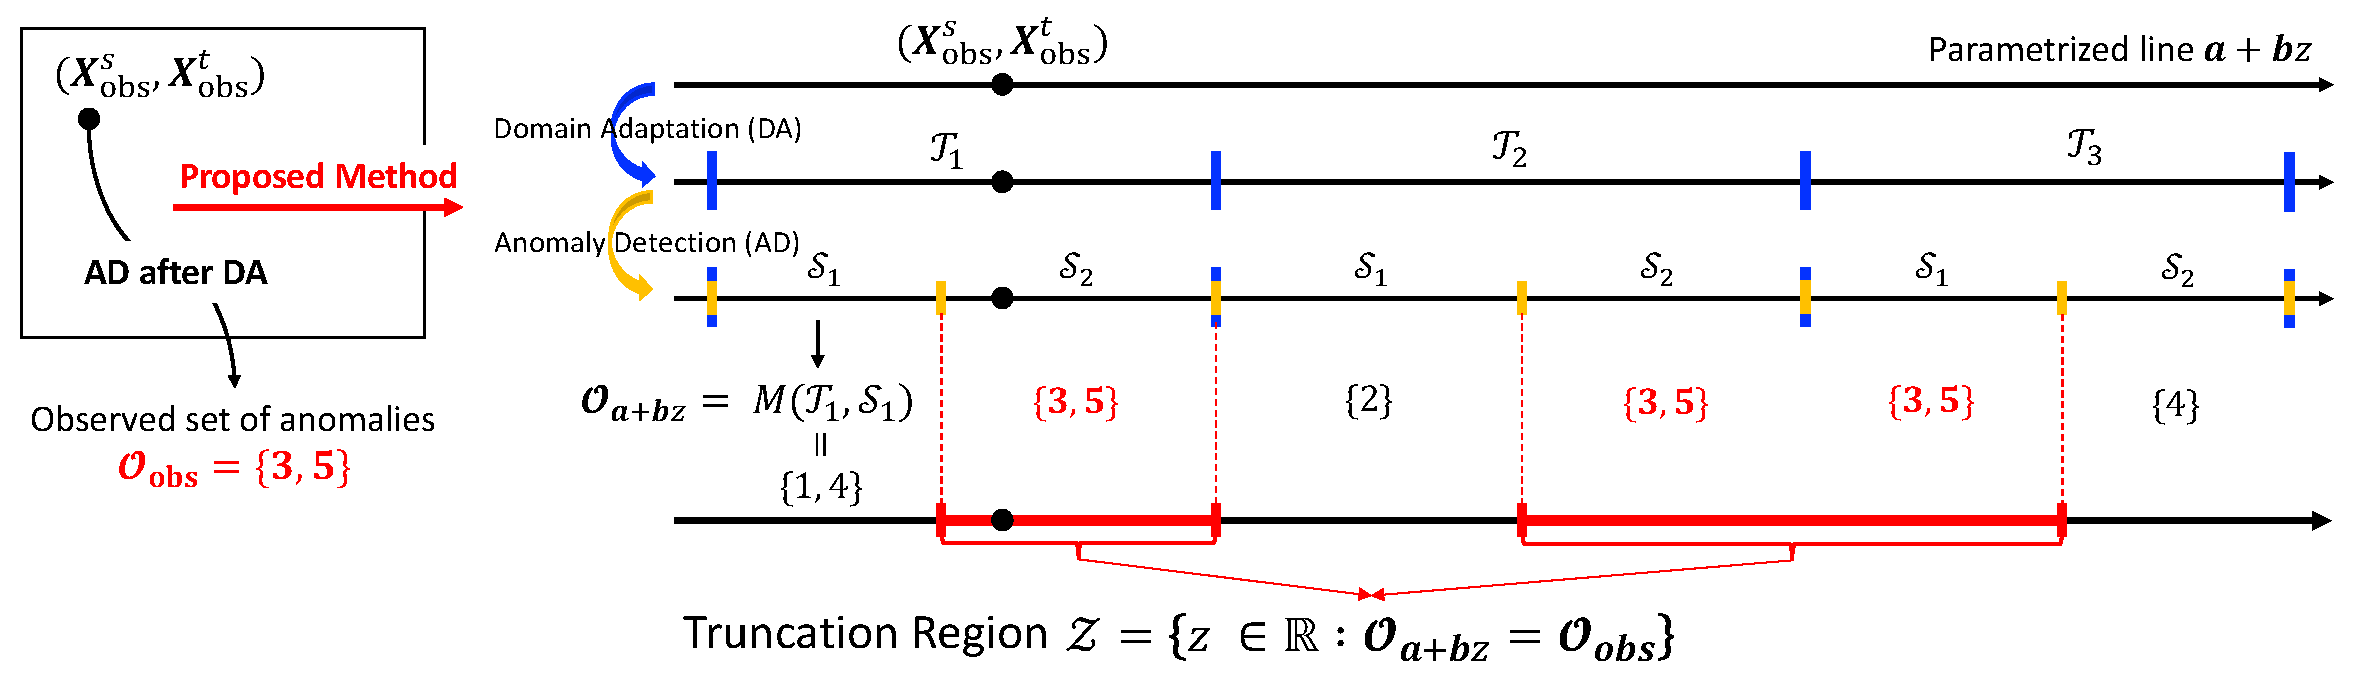
\includegraphics[width=\linewidth]{schematic_illustration.pdf} 
\caption{
\footnotesize 
A schematic illustration of the proposed method.
%
By applying AD after DA to the observed data, we obtain a set of anomalies.
%
Then, we parametrize the data with a scalar parameter $z$ in the dimension of the test statistic to identify the truncation region $\cZ$ whose data have the \emph{same} result of anomaly detection as the observed data.
%
Finally, the valid inference is conducted conditional on $\cZ$.
%
We utilize the concept of ``divide-and-conquer'' and introduce a hierarchical line search method for efficiently characterizing the truncation region $\cZ$.}
\label{fig:schematic_illustration}
\end{minipage}
\hspace{2pt}
\begin{minipage}{0.28\textwidth}
\centering
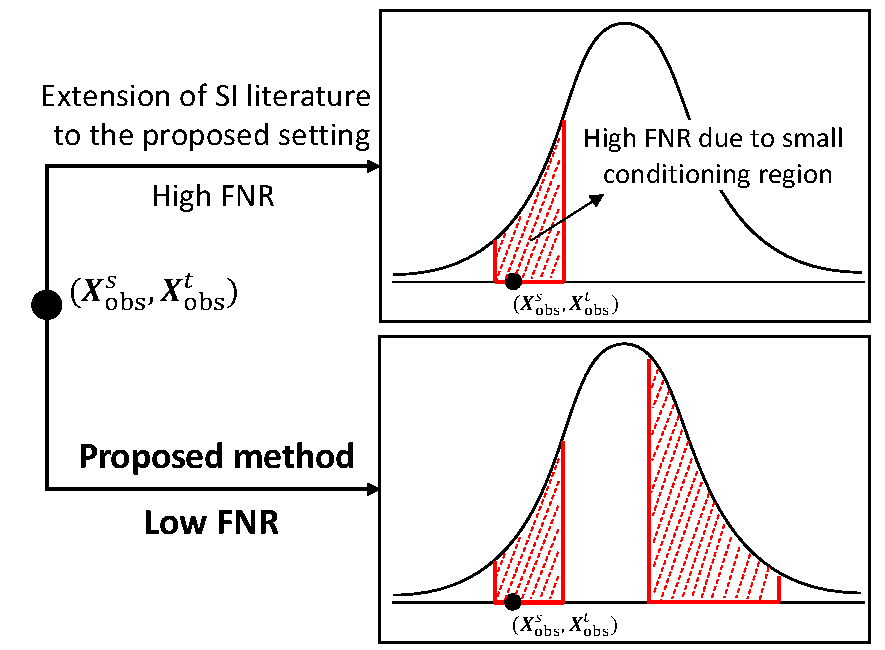
\includegraphics[width=.95\linewidth]{distributions} 
\caption{
\footnotesize 
If we leverage the idea of existing SI literature and apply to our setting, the FNR will be high due to small conditioning region by extra-conditioning. In contrast, the FNR is minimized with the proposed method.}
\label{fig:truncated_distributions}
\end{minipage}
\vspace{-8pt}
\end{figure*}



%
%\begin{figure*}[!t]
%\centering
%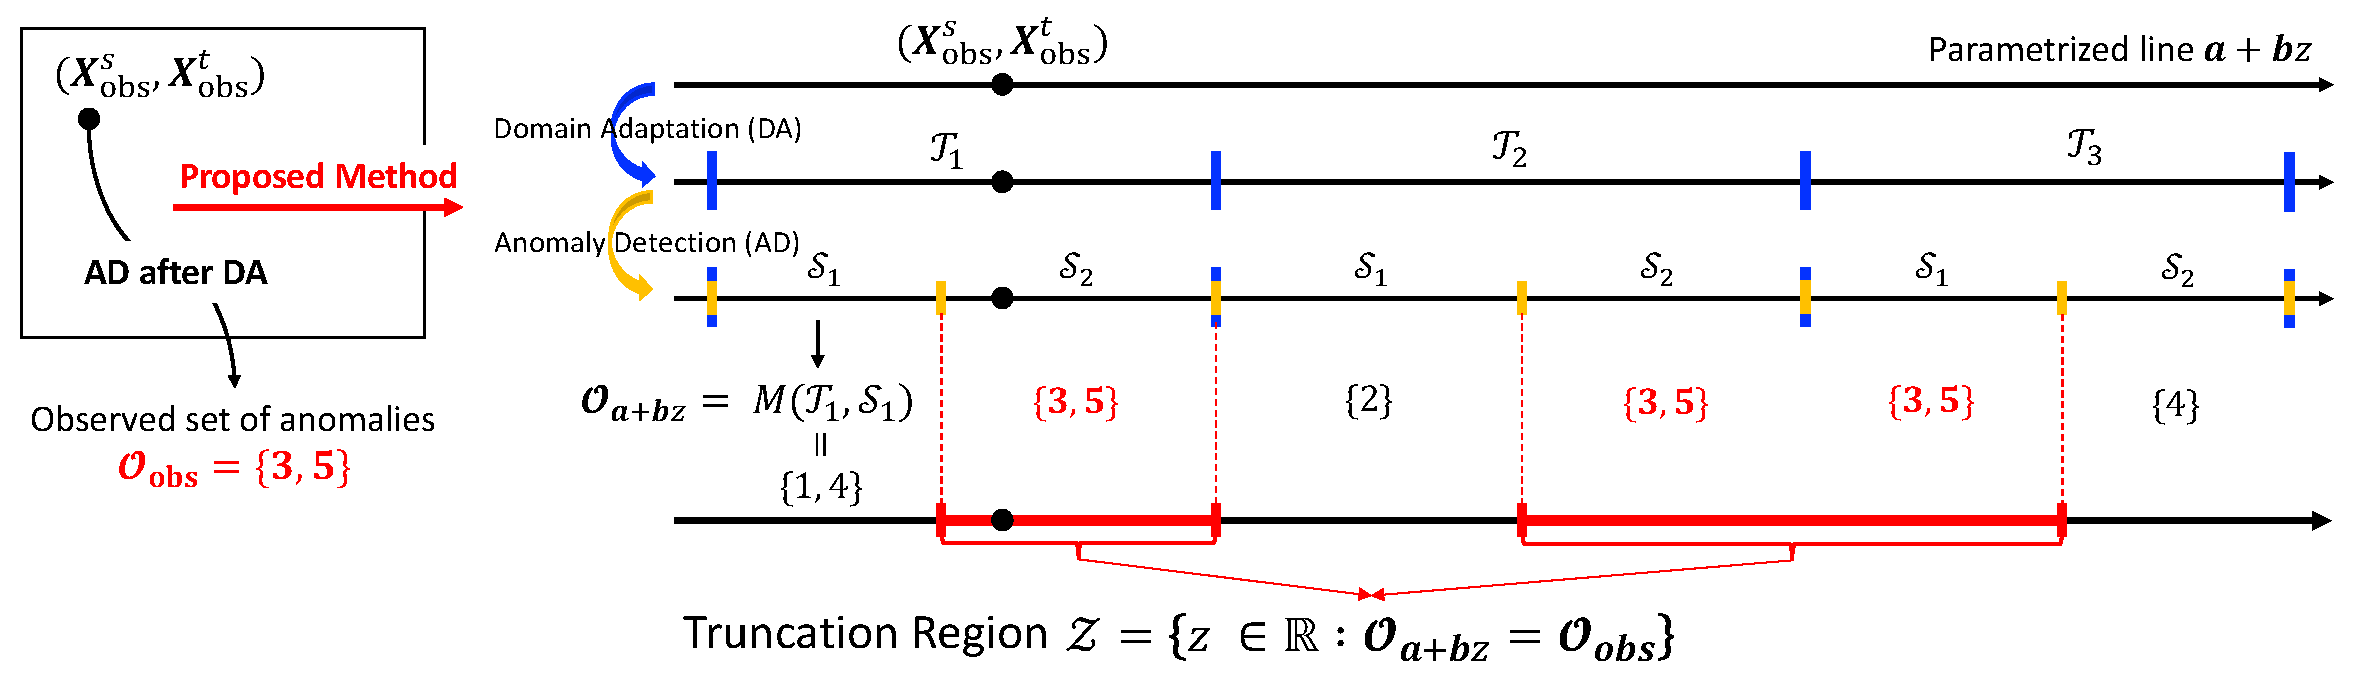
\includegraphics[width=.9\linewidth]{schematic_illustration.pdf} 
%\caption{A schematic illustration of the proposed method.
%%
%By applying AD after DA to the observed data, we obtain a set of anomalies.
%%
%Then, we parametrize the data with a scalar parameter $z$ in the dimension of the test statistic to identify the truncation region $\cZ$ whose data have the \emph{same} result of anomaly detection as the observed data.
%%
%Finally, the valid inference is conducted conditional on $\cZ$.
%%
%We utilize the concept of ``divide-and-conquer'' and introduce a hierarchical line search method for efficiently characterizing the truncation region $\cZ$.
%}
%\label{fig:schematic_illustration}
%\vspace{-5pt}
%\end{figure*}
%
%

\subsection{Conditional Data Space Characterization} \label{subsec:conditional_data_space}

We define the set of ${\bm X^s \choose \bm X^t } \in \RR^{n_s + n_t}$ that satisfies the conditions in \eq{eq:conditioning_event} as:
%
\begin{align} \label{eq:conditional_data_space}
	\hspace{-2.5mm}\cD = \left \{ 
	{\bm X^s \choose \bm X^t } \Big | ~
%	\begin{array}{l}
	\cO_{\bm X^s, \bm X^t}
	=
	\cO_{\rm obs}, 
	\cQ_{\bm X^s, \bm X^t}
	=
	\cQ_{\rm obs}
%	\end{array}
	\right \}. 
\end{align}
%
In fact, the conditional data space $\cD$ is \emph{a line} in $\RR^{n_s + n_t}$ as stated in the following lemma. 
%
\begin{lemma} \label{lemma:data_line}
The set $\cD$ in \eq{eq:conditional_data_space} can be rewritten using a scalar parameter $z \in \RR$ as follows:
%
\begin{align} \label{eq:conditional_data_space_line}
	\cD = \left \{ {\bm X^s \choose \bm X^t } = \bm a + \bm b z \mid z \in \cZ \right \},
\end{align}
%
where vector $\bm a = \cQ_{\rm obs}$, $\bm b$ is defined in \eq{eq:q_and_b}, and
%
\begin{align} \label{eq:cZ}
	\cZ = \Big \{ 
	z \in \RR 
	\mid 
	%\begin{array}{l}
	\cO_{\bm a + \bm b z} = \cO_{\rm obs}
	%\end{array}
	\Big \}.
\end{align}
Here, with a slight abuse of notation, 
$
\cO_{\bm a + \bm b z} = \cO_{{\bm X^s \choose \bm X^t }}
$
is equivalent to $\cO_{\bm X^s, \bm X^t}$.
\end{lemma}
%
\begin{proof}
The proof is deferred to Appendix \ref{appx:proof_lemma_data_line}.
%Based on the second condition in \eq{eq:conditional_data_space}, we have 
%%
%\begin{align*}
%	\cQ_{\bm X^s, \bm X^t} & =  \cQ_{\rm obs} \\ 
%	\Leftrightarrow 
%	\left ( 
%	I_{n_s + n_t} - 
%	\bm b
%	\bm \eta_j^\top \right ) 
%	{\bm X^s \choose \bm X^t}
%	& = 
%	\cQ_{\rm obs}\\ 
%	\Leftrightarrow 
%	{\bm X^s \choose \bm X^t}
%	& = 
%	\cQ_{\rm obs}
%	+ \bm b
%	\bm \eta_j^\top  
%	{\bm X^s \choose \bm X^t}.
%\end{align*}
%%
%By defining 
%$\bm a = \cQ_{\rm obs}$,
%$z = \bm \eta_j^\top {\bm X^s \choose \bm X^t}$, and incorporating the first condition of \eq{eq:conditional_data_space}, we obtain Lemma \ref{lemma:data_line}. 
\end{proof}


\begin{remark}
Lemma \ref{lemma:data_line} indicates that we need NOT consider the $(n_s + n_t)$-dimensional data space.
%
Instead, we need only consider the \emph{one-dimensional projected} data space $\cZ$ in \eq{eq:cZ}.
%
The fact of restricting the data to a line has been already implicitly exploited in \cite{lee2016exact}, and explicitly discussed in Sec. 6 of \cite{liu2018more}.
\end{remark}

\paragraph{Reformulation of the selective $p$-value.}
Let us consider a random variable and its observation:
%
\begin{align*}
	Z = \bm \eta_j^\top {\bm X^s \choose \bm X^t } \in \RR 
	~~ \text{and} ~~ 
	Z_{\rm obs} = \bm \eta_j^\top {\bm X^s_{\rm obs} \choose \bm X^t_{\rm obs} } \in \RR.
\end{align*}
%
%
%$Z = \bm \eta_j^\top {\bm X^s \choose \bm X^t } \in \RR$ and its observation $Z_{\rm obs} = \bm \eta_j^\top {\bm X^s_{\rm obs} \choose \bm X^t_{\rm obs} } \in \RR$,
% that satisfies 
%
%\begin{align*}
%	{\bm X^s \choose \bm X^t } = \bm a + \bm b Z 	
%	\quad \text{and} \quad 
%	{\bm X^s_{\rm obs} \choose \bm X^t_{\rm obs} } = \bm a + \bm b Z_{\rm obs},
%\end{align*}
%${\bm X^s \choose \bm X^t } = \bm a + \bm b Z$ and ${\bm X^s_{\rm obs} \choose \bm X^t_{\rm obs} } = \bm a + \bm b Z_{\rm obs}$.
Then, the selective $p$-value in (\ref{eq:selective_p}) can be rewritten as 
%
\begin{align} \label{eq:selective_p_reformulated}
	p^{\rm sel}_j = \mathbb{P}_{\rm H_{0, j}} \Big ( |Z| \geq |Z_{\rm obs}| \mid  Z \in \cZ \Big ).
\end{align}
%
Because $Z \sim \NN(0, \bm \eta_j^\top \Sigma \bm \eta_j)$ under the null hypothesis, $Z \mid Z \in \cZ$ follows a \emph{truncated} normal distribution. 
%
Once the truncation region $\cZ$ is identified, computation of the selective $p$-value in (\ref{eq:selective_p_reformulated}) is straightforward.
%
Therefore, the remaining task is to identify $\cZ$.

%============================


\subsection{Identification of Truncation Region $\cZ$} \label{subsec:identification_cZ}

As discussed in \S \ref{subsec:conditional_data_space}, to calculate the selective $p$-value \eq{eq:selective_p_reformulated}, we must identify the truncation region $\cZ$ in (\ref{eq:cZ}).
%
%To construct $\cZ$, we have to (a) compute $\cO_{\bm a + \bm b z}$ for all $z \in \RR$, and (b) identify the set of intervals of $z$ on which $\cO_{\bm a + \bm b z} = \cO_{\rm obs}$.
%%
%However, it seems intractable to obtain $\cO_{\bm a + \bm b z}$ for \emph{infinitely many values} of $z \in \RR$.
%
However, there is no direct way to identify $\cZ$.
%
To overcome the difficulty, we utilize the concept the ``\emph{divide-and-conquer}'' and introduce an approach (illustrated in Fig. \ref{fig:schematic_illustration}) to efficiently identify $\cZ$, described as follows:

$\bullet$ \textbf{Step 1 (extra-conditioning)}: breaking down the problem into multiple sub-problems by additionally conditioning the transportation for DA and all the steps of the AD after DA. Each sub-problem can be directly solved with a finite number of operations.
%, i.e., 
%%
%\begin{align*}
%	\cO_{\bm a + \bm b z} = \bigcup \limits_{x} \bigcup \limits_{x}
%	\Big \{ \cT_u =  \cT_{\bm a + \bm b z}, \cA_v =  \cA_{\bm a + \bm b z} \Big \} 
%\end{align*}

$\bullet$ \textbf{Step 2 (hierarchical line search)}: hierarchically combining multiple extra-conditioning steps and check the condition $\cO_{\bm a + \bm b z} = \cO_{\rm obs}$ to obtain $\cZ$.

Specifically, let us denote by $U$ a number of all possible transportations for DA along the parametrized line.
%
%After each transportation $\cT_u$, $u \in [U]$, the AD is conducted.
%
We denote by $V^u$ a number of all possible sets of steps performed by the AD algorithm after the $\cT_u$ transportation, $u \in [U]$.
%
The entire one-dimensional space $\RR$ can be decomposed as: 
\begin{align*}
	\RR
	& = 
	\bigcup \limits_{u \in [U]}
	\bigcup \limits_{v \in [V^u]}
	\Bigg \{ 
	\underbrace{
	z \in \RR 
	\mid 
	\cT_{\bm a + \bm b z} = \cT_u,
	\cS_{\bm a + \bm b z} = \cS_v}_{\text{a sub-problem of extra-conditioning}}
	\Bigg \},
\end{align*}
%
where $\cT_{\bm a + \bm b z}$ denotes the OT-based DA on $\bm a + \bm b z$, $\cS_{\bm a + \bm b z}$ denote a set of steps performed by the AD algorithm after DA.
%
Our goal is to search a set 
%
\begin{align}\label{eq:cW}
	\cW = 
	\Big \{ 
		(u, v) : \cM(\cT_u, \cS_v) = \cO_{\rm obs},
	\Big \}, 
\end{align}
%
for all $u \in [U], v \in [V^u]$, the function $\cM$ is defined as:
\[
\cM : \big (\cT_{\bm a + \bm b z}, \cS_{\bm a + \bm b z} \big ) \mapsto \cO_{\bm a + \bm b z}.
\]
%
Finally, the region $\cZ$ in \eq{eq:cZ} can be obtained as follows:
%
\begin{align}
	\hspace{-2mm}\cZ 
	& = \Big \{ 
	z \in \RR 
	\mid 
	\cO_{\bm a + \bm b z} = \cO_{\rm obs}
	\Big \} \nonumber \\ 
	%
	& = 
	\bigcup \limits_{(u, v) \in \cW}
	\Big \{ 
	z \in \RR 
	\mid 
	\cT_{\bm a + \bm b z} = \cT_u,
	\cS_{\bm a + \bm b z} = \cS_v
	\Big \}. \label{eq:cZ_new}
\end{align}
%
%\begin{align*}
%	\cU &= \Big \{ u \in [U] : 
%		\exists v \in [V^u] \text{ s.t. } \cM(\cT_u, \cS_v) = \cO_{\rm obs}
%	\Big \}, \\ 
%	\cV^u &= \Big \{ v \in [V^u] : \cM(\cT_u, \cS_v) = \cO_{\rm obs}
%	\Big \}, ~ \forall u \in [U],\\ 
%	\cM &: \big (\cT_{\bm a + \bm b z}, \cS_{\bm a + \bm b z} \big ) \mapsto \cO_{\bm a + \bm b z}.
%\end{align*}
%


\begin{algorithm}[!t]
\renewcommand{\algorithmicrequire}{\textbf{Input:}}
\renewcommand{\algorithmicensure}{\textbf{Output:}}
\begin{footnotesize}
 \begin{algorithmic}[1]
  \REQUIRE $\bm a, \bm b, z_{\rm min}, z_{\rm max}$
	\vspace{4pt}
	\STATE Initialization: $u = 1$, $v = 1$, $z_{u, v}  = z_{\rm min}$, $\cW = \emptyset$
	\vspace{4pt}
	\WHILE {$z_{u, v} < z_{\rm max}$}
		\vspace{4pt}
		\STATE $\cT_u \leftarrow$ DA on data $\bm a + \bm b z_{u, v}$
		\vspace{4pt}
		\STATE Compute $[L_u, R_u] = \cZ_u \leftarrow$ Lemma \ref{lemma:cZ_1} 
		\vspace{4pt}
		\WHILE {\emph{true}}
		\vspace{4pt}
		\STATE $\cS_v \leftarrow$ AD after DA on data $\bm a + \bm b z_{u, v}$
		\vspace{4pt}
		\STATE Compute $\cZ_v \leftarrow$ Lemma \ref{lemma:cZ_2} 
		\vspace{4pt}
		\STATE $[L_{u, v}, R_{u, v}] = \cZ_{u, v} \leftarrow \cZ_u \cap \cZ_v$ 
		\vspace{4pt}
		%
		\IF {$\cM(\cT_u, \cS_v) = \cO_{\rm obs}$}
		\vspace{4pt}
		\STATE $\cW \leftarrow \cW \cup \{ (u, v)\} $
		\vspace{4pt}
		\ENDIF
		%
		\vspace{4pt}
		%
		\IF {$R_{u, v} = R_u$}
		\vspace{4pt}
		\STATE $v \leftarrow 1$, $u \leftarrow u + 1$, $z_{u, v} = R_{u, v}$, \textbf{break}
		\vspace{4pt}
		\ENDIF
		%
%		\STATE \textbf{if} {$R_{u, v} = R_u$} \textbf{then} ${\rm break}$ \textbf{end if}
		%
		\vspace{4pt}
		\STATE $v \leftarrow v + 1$, $z_{u, v} = R_{u, v}$
		\vspace{4pt}
		\ENDWHILE	
%		\vspace{4pt}
%		\STATE $v \leftarrow 1$, $u \leftarrow u + 1$, $z_{u, v} = R_{u, v}$
		\vspace{4pt}
	\ENDWHILE
	\vspace{4pt}
  \ENSURE $\cW$ 
 \end{algorithmic}
\end{footnotesize}
\caption{{\tt hierachical\_line\_search}}
\label{alg:hierachical_line_search}
\end{algorithm}



\textbf{Extra-conditioning (step 1).} For any $u \in [U]$ and $v \in [V^u]$, we define the subset of one-dimensional projected dataset on a line for the extra-conditioning as:
%
\begin{align} \label{eq:cZ_extra_condition}
	\cZ_{u, v} = 
	\big \{z \in \RR 
	\mid 
	\cT_{\bm a + \bm b z} = \cT_u,
	\cS_{\bm a + \bm b z} = \cS_v 
	\big \}.
\end{align}
%
The extra-conditioning region can be re-written as:
%
\begin{align*}
	&\cZ_{u, v}  = \cZ_u \cap \cZ_v, \\ 
	\cZ_u  = 
	\big \{ 
	z
	\mid 
	\cT_{\bm a + \bm b z} &= \cT_u
	\big \},  ~ ~
	\cZ_v = 
	\big \{ 
	z 
	\mid 
	\cS_{\bm a + \bm b z} = \cS_v
	\big \}.
\end{align*}
%
\begin{lemma} \label{lemma:cZ_1}
The set $\cZ_u$ can be characterized by a set of quadratic inequalities w.r.t. $z$ described as follows:
\begin{align*}
	\cZ_u
%	& = 
%	\big \{ 
%	z \in \RR 
%	\mid 
%	\cT_{\bm a + \bm b z} = \cT_u
%	\big \} 
	= \Big \{ 
	z \in \RR 
	\mid 
	\bm w + \bm r z + \bm o z^2 \geq \bm 0
	\Big \},
\end{align*}
%
where vectors $\bm w$, $\bm r$, and $\bm o$ are defined in Appendix \ref{appx:proof_lemma_cZ_1}.
\end{lemma}

%\begin{proof}
%The proof is deferred to Appendix \ref{appx:proof_lemma_cZ_1}.
%\end{proof}

\begin{lemma} \label{lemma:cZ_2}
The set $\cZ_v$, which represents the set of operation performed by the MAD algorithm, can be characterized by a set of linear inequalities:
%
\begin{align} \label{eq:set_cZ_v}
	\cZ_v
%	& = 
%	\big \{ 
%	z \in \RR 
%	\mid 
%	\cT_{\bm a + \bm b z} = \cT_u
%	\big \} 
	= \Big \{ 
	z \in \RR 
	\mid 
	\bm p z \leq \bm q
	\Big \},
\end{align}
%
where vectors $\bm p$ and $\bm q$ are provided in Appendix \ref{appx:proof_lemma_cZ_2}.

\end{lemma}

%\begin{proof}
%The proof is deferred to Appendix \ref{appx:proof_lemma_cZ_2}.
%\end{proof}

The proofs of Lemmas \ref{lemma:cZ_1} and \ref{lemma:cZ_2} are deferred to Appendices \ref{appx:proof_lemma_cZ_1} and \ref{appx:proof_lemma_cZ_2}.
%
Since the definitions of $\bm w$, $\bm r$, $\bm o$, $\bm p$, and $\bm q$ are complex and require extensive descriptions, we deferred them to the Appendices.
%
Briefly speaking, they are used for ensuring that the transportation and all the steps of the AD after DA remains the same for all $z \in \cZ_{u, v}$.
%
Lemmas \ref{lemma:cZ_1} and \ref{lemma:cZ_2} indicate that $\cZ_u$ and $\cZ_v$ can be \emph{analytically obtained} by solving the systems of quadratic and linear inequalities, respectively.
%
After computing $\cZ_u$ and $\cZ_v$, the extra conditioning region $\cZ_{u, v}$ in \eq{eq:cZ_extra_condition} is obtained by $\cZ_{u, v}  = \cZ_u \cap \cZ_v$.
%
As mentioned in \S \ref{sec:problem_setup}, our proposed CAD-AD can be applied to other AD algorithms whose operations can be characterized by sets of linear/quadratic inequalities (e.g., least absolute deviations, Huber regression).


\begin{remark}
The selective $p$-value computed with the extra-conditioning region $\cZ_{u, v}$ is still valid and this fact is well-known in the literature of conditional SI.
%
The computation of $\cZ_{u, v}$ can be considered as an extension of the methods presented in \cite{lee2016exact} and \cite{duy2021exact} into our proposed setting.
%
However, the major drawback of this case is that the TPR is low, i.e., the FNR is high.
%
Therefore, we introduce the line search step to remove the extra-conditioning for the purpose of minimizing the FNR.
%
The illustration is shown in Fig. \ref{fig:truncated_distributions}.
 
\end{remark}



\textbf{Hierarchical line search (step 2).}
Our strategy is to identify $\cW$ in \eq{eq:cW} by repeatedly applying OT-based DA and MAD after DA  to a sequence of datasets $\bm a + \bm b z$ within sufficiently wide range of $z \in [z_{\rm min}, z_{\rm max}]$\footnote{We set $z_{\rm min} = -20\sigma$ and $z_{\rm max} = 20 \sigma$, $\sigma$ is the standard deviation of the distribution of the test statistic, because the probability mass outside this range is negligibly small.}.
%
For simplicity, we consider the case in which $\cZ_u$ is an interval \footnote{If $\cZ_u$ is a union of intervals, we can select the interval containing the data point that we are currently considering.}. 
%
Since $\cZ_v$ is also an interval, $\cZ_{u, v}$ is an interval.
%
We denote $\cZ_u = [L_u, R_u]$ and $\cZ_{u, v} = [L_{u, v}, R_{u, v}]$.
%
The hierarchical line search procedure can be summarized in Algorithm \ref{alg:hierachical_line_search}.
%
After obtaining $\cW$ by Algorithm \ref{alg:hierachical_line_search}.
%
We can compute $\cZ$ in \eq{eq:cZ_new}, which is subsequently used to obtain the proposed selective $p$-value in \eq{eq:selective_p_reformulated}.
%
The entire steps of the proposed CAD-DA method is summarized in Algorithm \ref{alg:cad_da}.



\begin{algorithm}[!t]
\renewcommand{\algorithmicrequire}{\textbf{Input:}}
\renewcommand{\algorithmicensure}{\textbf{Output:}}
\begin{footnotesize}
 \begin{algorithmic}[1]
  \REQUIRE $\bm X^s_{\rm obs}, \bm X^t_{\rm obs}, z_{\rm min}, z_{\rm max}$
	\vspace{4pt}
	\STATE $\cO_{\rm obs} \leftarrow$ AD after DA on $\big \{ \bm X^s_{\rm obs}, \bm X^t_{\rm obs} \big \} $
	\vspace{4pt}
	\FOR {$j \in \cO_{\rm obs}$}
		\vspace{4pt}
		\STATE Compute $\bm \eta_j \leftarrow$ Eq. \eq{eq:eta_j}, $\bm a$ and $\bm b \leftarrow$ Eq. \eq{eq:conditional_data_space_line}
		\vspace{4pt}
		\STATE $\cW \leftarrow$ {\tt hierachical\_line\_search} ($\bm a, \bm b, z_{\rm min}, z_{\rm max}$)
		\vspace{4pt}
		\STATE $p^{\rm sel}_j \leftarrow$  Eq. \eq{eq:selective_p_reformulated} with $\cZ \leftarrow$ Eq. \eq{eq:cZ_new}
		\vspace{4pt}
	\ENDFOR
	\vspace{4pt}
  \ENSURE $\big \{ p^{\rm sel}_j \big \}_{j \in \cO_{\rm obs}}$ 
 \end{algorithmic}
\end{footnotesize}
\caption{{\tt CAD-DA}}
\label{alg:cad_da}
\end{algorithm}



%\vspace{-2pt}
\subsection{Extension to Multi-Dimension} \label{subsec:extension}
%\vspace{-3pt}
In this section, we generalize the problem setup and the proposed method in multi-dimension. 
%
We consider two random sets $X^s \in \RR^{n_s \times d}$ and $X^t \in  \RR^{n_t \times d}$ of $d$-dimensional vectors 
%
%\begin{align*}
%	  X^s &= \big (\bm X^s_{1}, \ldots, \bm X^s_{n_s} \big )^\top  \in \RR^{n_s \times d},  \\ 
%	X^t &= \big (\bm X^t_{1}, \ldots, \bm X^t_{n_t} \big )^\top \in  \RR^{n_t \times d},
%\end{align*}
%
which are random samples from
%
%\begin{footnotesize}
\begin{align*}
	{\rm {vec}} (X^s) &\sim \NN \Big ({\rm vec} (M^s), ~ \Sigma^s_{{\rm vec} (X^s)} \Big ), \\
	{\rm {vec}} (X^t) &\sim \NN \Big ({\rm vec} (M^t), ~ \Sigma^t_{{\rm vec} (X^t)} \Big ),
\end{align*}
%\end{footnotesize}
%
where ${\rm vec}(\cdot)$ is an operator that transforms a matrix into a vector with concatenated rows, $M^s$ and $M^t$ are signal matrices that are unknown, $\Sigma^s_{{\rm vec} (X^s)}$ and $\Sigma^t_{{\rm vec} (X^t)}$ are variance matrices that are known. %or estimated from independent data.
%
%The cost matrix between $X^s$ and $X^t$ is defined as 
%\begin{align*} %\label{eq:cost_matrix_l_2}
%	C( X^s,  X^t) 
%	& = \left[ \sum \limits_{\kappa=1}^d (X_{i, \kappa}^s - X_{j, \kappa}^t)^2 \right ]_{ij} \in \RR^{n_s \times n_t}.
%\end{align*}
%
After obtaining $\hat{T}$ by solving the OT problem, %with $C( X^s,  X^t)$, 
we obtain 
%
$\tilde{X}^s = n_s \hat{T} X^t$.
%
Then, the AD result after DA is:
%
\begin{align*}
	\cA: \big \{ \tilde{X}^s, X^t \big \} 
		\mapsto
		\cO \in [n_t].
\end{align*}
%
For $j \in \cO$, we consider the following hypotheses:
%
\begin{align*}
	{\rm H}_{0, j}:  M^t_{j, \kappa} = \bar{ M}^t_{- \cO, \kappa}
	\quad
	\text{vs.}
	\quad 
	{\rm H}_{1, j}:  M^t_{j, \kappa} \neq \bar{M}^t_{- \cO, \kappa},
\end{align*}
%
for all $\kappa \in [d]$, 
%$\bar{M}^t_{- \cO, \kappa}$ is defined as:
%
$
	\bar{M}^t_{- \cO, \kappa} = 
	\frac{1}{n_t - |\cO|} \sum \limits_{\ell \in [n_t] \setminus \cO}
	M^t_{\ell, \kappa}.
$

The test-statistic is then can be defined as:
%
\begin{align} \label{eq:test_statistic_mul}
	\Gamma_j = \sum_{\kappa \in [d]}
	|X^t_{j, \kappa} - \bar{X}^t_{- \cO, \kappa}| 
\end{align}
%
In order to compute the valid $p$-values, % for the AD results, 
we consider the following conditional distribution of the test statistic:
%
\begin{align} \label{eq:conditional_distribution_mul}
	\mathbb{P} \Big ( 
	\Gamma_j
	\mid
	\cO_{X^s, X^t}
	=
	\cO_{\rm obs}, ~
	\cI_{X^s, X^t} 
	=
	\cI_{\rm obs}
	\Big ),
\end{align}
%
where $\cI_{X^s, X^t}$ is a set of all the signs of the subtractions in \eq{eq:test_statistic_mul}.
%
By extending the techniques in \S \ref{subsec:conditional_data_space} and \S \ref{subsec:identification_cZ}, % into the setting of multi-dimension, 
the conditional space in \eq{eq:conditional_distribution_mul} can be obtained which is subsequently used to compute the $p$-value.


%\paragraph{Current limitations and other extensions.}


















